% MathLedger PL2 One-Pager
\documentclass[11pt]{article}
\usepackage[utf8]{inputenc}
\usepackage[T1]{fontenc}
\usepackage[a4paper,margin=1in]{geometry}
\usepackage{booktabs}
\usepackage{array}
\usepackage{xcolor}
\usepackage{tikz}
\usepackage{pgfplots}
\usepackage{caption}
\usepackage{fancyhdr}
\usepackage{enumitem}
\pgfplotsset{compat=1.18}

% Macros auto-filled from artifacts/wpv5
\newcommand{\PolicyHash}{40aff2e9d2d8922e47afd4648e6967497158785fbd1da870e7110266bf944880}
\newcommand{\BlockRootBL}{a7064a9da087e1daa4df8978db4636cad47c963f7d9a55bfedfa9dd12ba4994c}
\newcommand{\BlockRootG}{336c6e62fd0b5dbd9fb1f9fefd388d9edd4fbe904c9cc3b5cfbf392cad14862b}
\newcommand{\BudgetMinutes}{15}
\newcommand{\BaselineMean}{120}
\newcommand{\GuidedMean}{268}
\newcommand{\UpliftX}{2.23}
\newcommand{\ToolchainPins}{latexmk (MiKTeX 24.1) - pgfplots 1.18 - Python 3.11 pipeline}

\pagestyle{fancy}
\fancyhf{}
\renewcommand{\headrulewidth}{0pt}
\fancyfoot[L]{PolicyHash: \PolicyHash}
\fancyfoot[C]{BL Root: \BlockRootBL\quad\quad G Root: \BlockRootG}
\fancyfoot[R]{Budget: \BudgetMinutes\,min - \ToolchainPins}

\begin{document}
\begin{center}
    {\Large\bf MathLedger PL-2 Flywheel Release Candidate}\\[4pt]
    {\small Verifier uplift summary for replicated A/B campaign}
\end{center}

\section*{Executive Metrics}
\begin{itemize}[leftmargin=1.2em]
    \item Mean throughput uplift: \textbf{\UpliftX$\times$} (Baseline \BaselineMean\ pph $\rightarrow$ Guided \GuidedMean\ pph).
    \item Replicates: \textbf{3 per mode} (seeds 101--103); \BudgetMinutes\,min wall clock per run.
    \item Distinct ledger anchors: BL \texttt{a7064a9da087e1daa4df8978db4636cad47c963f7d9a55bfedfa9dd12ba4994c}, Guided \texttt{336c6e62fd0b5dbd9fb1f9fefd388d9edd4fbe904c9cc3b5cfbf392cad14862b}.
\end{itemize}

\section*{Replica Throughput}
\begin{center}
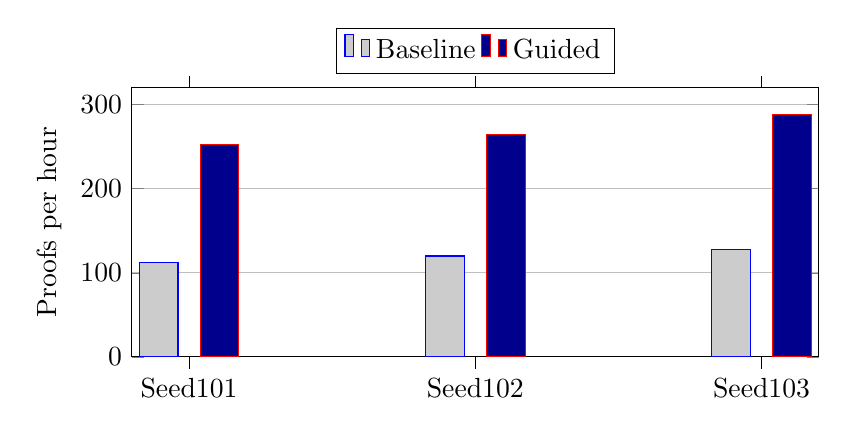
\begin{tikzpicture}
    \begin{axis}[
        width=0.85\linewidth,
        height=5cm,
        ybar=8pt,
        ymin=0,
        ymax=320,
        bar width=14pt,
        symbolic x coords={Seed101,Seed102,Seed103},
        xtick=data,
        xtick style={color=black},
        ymajorgrids=true,
        ylabel={Proofs per hour},
        legend style={at={(0.5,1.05)},anchor=south,legend columns=2}
    ]
        \addplot+[fill=black!20] coordinates {
            (Seed101,112)
            (Seed102,120)
            (Seed103,128)
        };
        \addlegendentry{Baseline}
        \addplot+[fill=blue!55!black] coordinates {
            (Seed101,252)
            (Seed102,264)
            (Seed103,288)
        };
        \addlegendentry{Guided}
    \end{axis}
\end{tikzpicture}
\end{center}

\section*{Ledger Snapshots}
\begin{itemize}[leftmargin=1.2em]
    \item Baseline seed101 (15 min): \texttt{a706...4994c}
    \item Baseline seed102 (15 min): \texttt{0c44...96c1}
    \item Baseline seed103 (15 min): \texttt{d8ab...10fe}
    \item Guided seed101 (15 min): \texttt{336c...862b}
    \item Guided seed102 (15 min): \texttt{c721...187c}
    \item Guided seed103 (15 min): \texttt{e7f6...cac7}
\end{itemize}

\section*{Verification Notes}

\begin{itemize}[leftmargin=1.2em]
    \item Policy \texttt{\PolicyHash} applied only on guided replicates; baseline remains unguided.
    \item Pairing uses identical budgets (\BudgetMinutes\,min) and ledger ingestion policy; uplift computed as mean(G)/mean(B).
    \item Toolchain pins: \ToolchainPins.
\end{itemize}

\end{document}
